\documentclass{softwaremanual}

\usepackage{titling}

% Figures and controlling packages
\usepackage{float}
\usepackage{wrapfig}

% logo for the title page
\newcommand{\swlogo}{{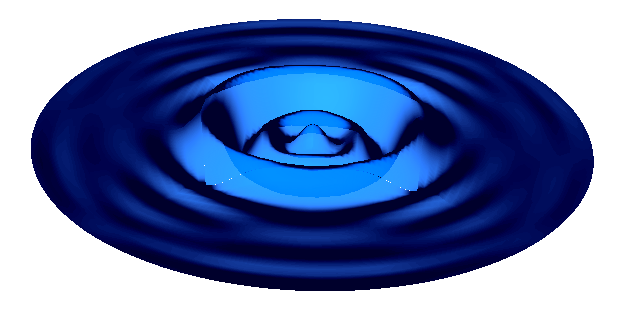
\includegraphics[width=0.25\textwidth]{images/shallowWater.png}}
}


\author{Joseph Schoonover}
\date{}

\begin{document}
\frontmatter
% Doing a custom title-page
\begin{titlingpage}
    
        \vspace*{2cm}

   % Setup up the main and sub-titles with the logo
   {\fontfamily{cmss}\selectfont
   \begin{center}
     \HUGE{\textbf{ Spectral Element Libraries in Fortran (SELF) }}\\

     \huge{\textbf{\textcolor{blue}{Shallow Water Equations}}}
   \end{center}
    }    
 
        \vspace{1cm}
        
        \begin{center}
         \swlogo
        \end{center}
        
        \vspace{2cm}
        
     \begin{center}
     
        %Do a subtitle here if you like
        {\fontfamily{cmss}\selectfont
        \huge{
           Reference Manual
        }
        
        \vspace{1.5cm}
        
        % Enter the author's name
        \textbf{
        \large{
           \theauthor 
         }}}
        
        \vfill
        
        
     \end{center}
        
    
\end{titlingpage}


{\fontfamily{cmss}\selectfont
\tableofcontents
}
\mainmatter

% Special Style
\pagestyle{myheadings}

\chapter{Equations and Discretization}
The inviscid shallow water equations are a system of coupled partial differential equations that is hyperbolic. The Nodal Discontinuous Galerkin Spectral Element Method (NDGSEM) is well suited for hyperbolic systems. It is highly accurate through its use of arbitrarily high order piecewise polynomial representation of the approximated solution and geometry. It is well known for exhibiting minimal numerical dispersion and dissipation errors. It additionally allows for a flexible treatment of the geometry through the use of a structured or unstructured arrangement of \textit{spectral elements} that can represent boundaries through high order polynomial interpolants. The discretization yields dense and local matrix-vector multiplies for computing derivatives and only requires nearest neighbor communication to calculate exchanges between elements. This last property makes the NDGSEM trivial to parallelize. For these reasons, the NDGSEM is applied to the shallow water equation systems \eqref{eq:conservative}, \eqref{eq:skewsymmetric}, and \eqref{eq:linear} to demonstrate its accuracy and scalability for a system of equations that hold many of the important dynamics in geophysics. 

\section{Flavors of the Shallow Water Equations}
The shallow water equations can be written in either ``conservative'' (Eqs. \ref{eq:conservative}) or ``skew-symmetric'' (Eqs. \ref{eq:skewsymmetric}) form :
\begin{subequations}
\begin{align}
U_t  + \nabla \cdot \left( \frac{\vec{U}U}{h + \eta} + g \left(h + \frac{\eta}{2} \right)\eta\hat{x} \right) - fV &= g\eta h_x  + q_U\\
V_t  + \nabla \cdot \left( \frac{\vec{U}V}{h + \eta} + g \left(h + \frac{\eta}{2} \right)\eta\hat{y} \right) + fU &= g\eta h_y + q_V\\
\eta_t + \nabla \cdot \vec{U} &= q_\eta
\end{align}\label{eq:conservative}
\end{subequations}

\begin{subequations}
\begin{align}
u_t  + \nabla \cdot \left( (e + p)\hat{x} \right) - (f+\zeta)v &=  q_u\\
v_t  + \nabla \cdot \left( (e + p)\hat{y} \right) + (f+\zeta)u &=  q_v\\
p_t + \nabla \cdot ( (gh+p)\vec{u} ) &= q_p
\end{align}\label{eq:skewsymmetric}
\end{subequations}
For either system, and throughout the rest of this documentation the symbols have the following meaning :
\begin{itemize}
\item[] $x, y$ : Cartesian coordinate positions ($Length$)
\item[] $t$    : Time
\item[] $U, V$ : The $x,y$ components of the the fluid \textit{transport} ($\frac{Length^2}{Time}$) 
\item[] $H$    : The total fluid thickness, bathymetric plus free surface ($Length$)
\item[] $h$    : Resting fluid depth, the fluid bathymetry ($Length$)
\item[] $g$    : Local acceleration of gravity ($\frac{Length}{Time^2}$)
\item[] $f$    : Coriolis parameter ($Time^{-1}$)
\item[] $u,v$  : The $x,y$ components of the \textit{depth average} fluid velocity ($\frac{Length}{Time}$)
\item[] $e$    : The kinetic energy of the depth averaged velocity field ($\frac{Length^2}{Time^2}$)
\item[] $p$    : Barotropic pressure, the product of gravitational acceleration and free surface anomaly ($\frac{Length^2}{Time^2}$)
\item[] $\zeta$ : The relative vorticity of the depth averaged velocity field ($Time^{-1}$)
\item[] $q_{\phi}$ : Any additional non-conservative source for the variable $\phi$ ($\frac{\phi}{Time}$) 
\end{itemize}

The linear shallow water equations \eqref{eq:linear} are given as
\begin{subequations}
\begin{align}
u_t  + \nabla \cdot \left( p\hat{x} \right) - fv &=  q_u\\
v_t  + \nabla \cdot \left( p\hat{y} \right) + fu &=  q_v\\
p_t + \nabla \cdot ( gh\vec{u} ) &= q_p
\end{align}\label{eq:linear}
\end{subequations}

Any flavor of the shallow water equations arise from a conservation law, and as such, \eqref{eq:conservative}, \eqref{eq:skewsymmetric}, or \eqref{eq:linear} can be written in the compact form
\begin{equation}
\vec{s} + \nabla \cdot \vec{f} = \vec{q}. \label{eq:conservationlaw}
\end{equation}
The solution vector is represented by $\vec{s}$, $\vec{f}$ is a conservative flux tensor, and $\vec{q}$ is a vector of non-conservative source terms. The derivation of the discrete equations is presented through a discretization of \eqref{eq:conservationlaw}. 

\section{Nodal Discontinuous Galerkin Discretization}
The NDGSEM discretizes \eqref{eq:conservationlaw} in its weak form. The physical space over which \eqref{eq:conservationlaw} is solved is denoted by $\Omega$. Solutions to \eqref{eq:conservationlaw} are real functions that are piecewise continuous on $\Omega$. This space of functions is denoted $\mathbb{C}_0(\Omega)$, and is defined mathematically
\begin{equation}
\mathbb{C}_0(\Omega) \equiv \left\lbrace \phi(\vec{x}) \in \mathbb{R} : \int_{\Omega} \phi^2 d\Omega < \infty \right\rbrace,
\end{equation}
\textit{`` the set of all functions $\phi$ that are square integrable over the physical space $\Omega$ ''}.

$\mathbb{C}_0(\Omega)$ has an inner product associated with it, defined by
\begin{equation}
(u,v) = \int_{\Omega} uv \hspace{1mm} d\Omega. \label{eq:innerproduct}
\end{equation}
From the definition of the inner product, the \textit{induced norm} of a function that is in $\mathbb{C}_0(\Omega)$ is defined as
\begin{equation}
||u|| = \sqrt{(u,u)}.\label{eq:norm}
\end{equation}
Similar to vectors, the inner-product \eqref{eq:innerproduct} is a measure of the ``common information'' between $u$ and $v$. Two functions are said to be \textit{orthogonal} if
\begin{equation}
(u,v) = 0. \label{eq:orthogonality}
\end{equation}

Any piecewise continuous function can be represented as a linear combination of a \textit{basis functions} that span $\mathbb{C}_0(\Omega)$. The weak form of \eqref{eq:conservationlaw} is obtained by taking the inner product of \eqref{eq:conservationlaw} with each basis function of $\mathbb{C}_0(\Omega)$,  
\begin{equation}
(\vec{s}_t,\phi) + (\nabla \cdot \vec{f}, \phi) = (\vec{s},\phi), \hspace{3mm} \forall \phi \in \mathbb{C}_0(\Omega) \label{eq:step1}
\end{equation}
In Eqs. \eqref{eq:conservative}, \eqref{eq:skewsymmetric}, and \eqref{eq:linear}, the conservative flux depends on the solution. In \eqref{eq:step1}, the divergence of the flux  requires that the solution is at least once differentiable. This differentiability constraint is relaxed in the weak form by performing integration by parts, which moves the differentiability criteria onto the basis function ($\phi$). Performing integrations by parts gives
\begin{equation}
(\vec{s}_t,\phi) + \oint_{\partial \Omega}\phi \vec{f} \cdot \hat{n} \hspace{1mm} dS - ( \vec{f},\nabla \phi) = (\vec{s},\phi), \hspace{3mm} \forall \phi \in \mathbb{C}_0(\Omega) \label{eq:weakform}
\end{equation}


 To develop a discrete set of equations, all of $\mathbb{C}_0(\Omega)$ is approximated by piecewise continuous polynomials of degree $N$, a space we denote $\mathbb{P}^N$. The solution, conservative flux, and the non-conservative source term are approximated by a linear combination of a suitable basis for $\mathbb{P}^N$. Since the solution is piecewise continuous, the domain $\Omega$, is decomposed into a set of non-overlapping elements $\Omega_l$. The integration is  broken into integration over each of the elements,
  \begin{equation}
 \sum_{\kappa=0}^{nEl} \left\lbrace \int_{\Omega_\kappa} (\vec{s}_t + \vec{q} )\phi_\kappa \hspace{1mm} d\Omega_\kappa  - \int_{\Omega_l} \vec{f} \cdot \nabla \phi_\kappa \hspace{1mm} d\Omega_\kappa + \oint_{\partial \Omega^\kappa} \phi_\kappa \vec{f}\cdot \hat{n} \hspace{1mm} d A_\kappa = 0 \right\rbrace, \hspace{3mm} \forall \phi_\kappa \in \mathbb{P}^n. \label{eq:weak-decomp}
  \end{equation}

In the \textit{Discontinuous} Galerkin approximation, the $\phi_l$ are identically zero outside of the $l^{th}$ element, so that the contributions from each element are decoupled (except for the element boundary integration). This feature of DG is called \textit{compact support}. Again, the solution, flux, and source are approximated by a polynomial of degree $N$. We choose to write each term as a linear combination of polynomial basis function; here the Lagrange interpolating polynomials are used,
\begin{subequations}
    \begin{align}
    \vec{s} &\approx I^N[\vec{s}] = \vec{S} =  \sum_{i,j=0}^N \vec{S}_{i,j} l_i(\xi^1) l_j(\xi^2) \\
    \vec{q} &\approx I^N[\vec{q}]= \vec{Q} = \sum_{i,j=0}^N \vec{Q}_{i,j} l_i(\xi^1) l_j(\xi^2) \\
    \vec{f} &\approx I^N[\vec{f}] =\vec{F}= \sum_{i,j=0}^N \vec{F}_{i,j} l_i(\xi^1) l_j(\xi^2)
    \end{align}
 \end{subequations}


The basis functions for $\mathbb{P}^N$ are chosen as each of the Lagrange interpolating polynomials, 
 \begin{equation}
 \phi_{m,n} = l_m(\xi^1) l_n(\xi^2)
 \end{equation}
 With this, equation \eqref{eq:weak-decomp} becomes
   \begin{equation}
  \int_{\Omega^\xi} (\vec{S}^\kappa_t + \vec{Q}^\kappa) \phi_{m,n}  \hspace{1mm} d\Omega^\xi  - \int_{\Omega^\xi} \vec{F}^\kappa \cdot \nabla_{\vec{\xi}} \phi_{m,n}   \hspace{1mm} d\Omega^\xi + \oint_{\partial \Omega^\xi} \phi_{m,n}  \vec{F}^{\kappa,*}  \cdot \hat{n} \hspace{1mm} d A^\xi = 0, \hspace{2mm} m,n=0,1,...,N  \label{eq:weak-decomp-basis}
  \end{equation}
  
The final step is to replace the integrals in \eqref{eq:approx_mappedWeakForm} with discrete quadrature. For this we use the Legendre-Gauss quadrature, which yields exact integration for each term in \eqref{eq:approx_mappedWeakForm}. Additionally, the interpolation nodes are specified as the Legendre-Gauss nodes, which simplifies the integration.


 \begin{equation}
 \begin{split}
 \left( J_{m,n} \vec{S}_{m,n} \right)_t =  &-\left[\sum_{i=0}^{N}\hat{D}^{(\xi^1)}_{m,i} \tilde{F}^{(\xi^1)}_{i,n}   + \left( \frac{ l_m(1)}{w^{(\xi^1)}_m} \tilde{F}^{*}(1,\xi^2_n) - \frac{ l_m(-1)}{w^{(\xi^1)}_m} \tilde{F}^{*}(-1,\xi^2_n) \right) \cdot \hat{\xi^1} \right] \\
  &-\left[ \sum_{j=0}^{N}\hat{D}^{(\xi^2)}_{n,j} \tilde{F}^{(\xi^2)}_{m,j}  + \left( \frac{l_n(1)}{w^{(\xi^2)}_n} \tilde{F}^{*}(\xi^1_m,1)  -  \frac{l_n(-1)}{w^{(\xi^2)}_n} \tilde{F}^{*}(\xi^1_m,-1) \right)\cdot \hat{\xi^2}  \right] \\ 
 &+ J_{m,n}\vec{Q}_{m,n}; \hspace{5mm} m,n=0,1,...,N
\end{split} \label{eq:discrete2d_system} 
 \end{equation}

Each element can support curvilinear geometry. Define the mapping from physical space $\vec{x}$ to computational space $\vec{\xi}$ using
  \begin{equation}
  \vec{x} = \vec{x}(\vec{\xi}).\label{eq:mapping}
  \end{equation}
In this case, the solution and the source term are weighted by the Jacobian of the mapping and the flux is rotated to the \textit{contravariant} flux. Appendix \ref{chap:GeometryTheory} provides the details on the metric terms that are introduced along with the form of the divergence, gradient, and curl under such a mapping.

 Computing the divergence of the conservative flux in this framework can be viewed as calculating a sequence of derivatives in each computational direction. Two steps are required to compute the derivative in each direction. The first is an internal matrix-vector multiply, and the second is computing the weighted Riemann fluxes at the element boundaries. The latter is the only step which requires element-to-element communication. The approximate fluxes are now presented for the systems \eqref{eq:conservative}, \eqref{eq:skewsymmetric}, and \eqref{eq:linear}.

\subsection{Riemann Flux}
\textit{This section needs some attention!}
\begin{figure}
\begin{center}
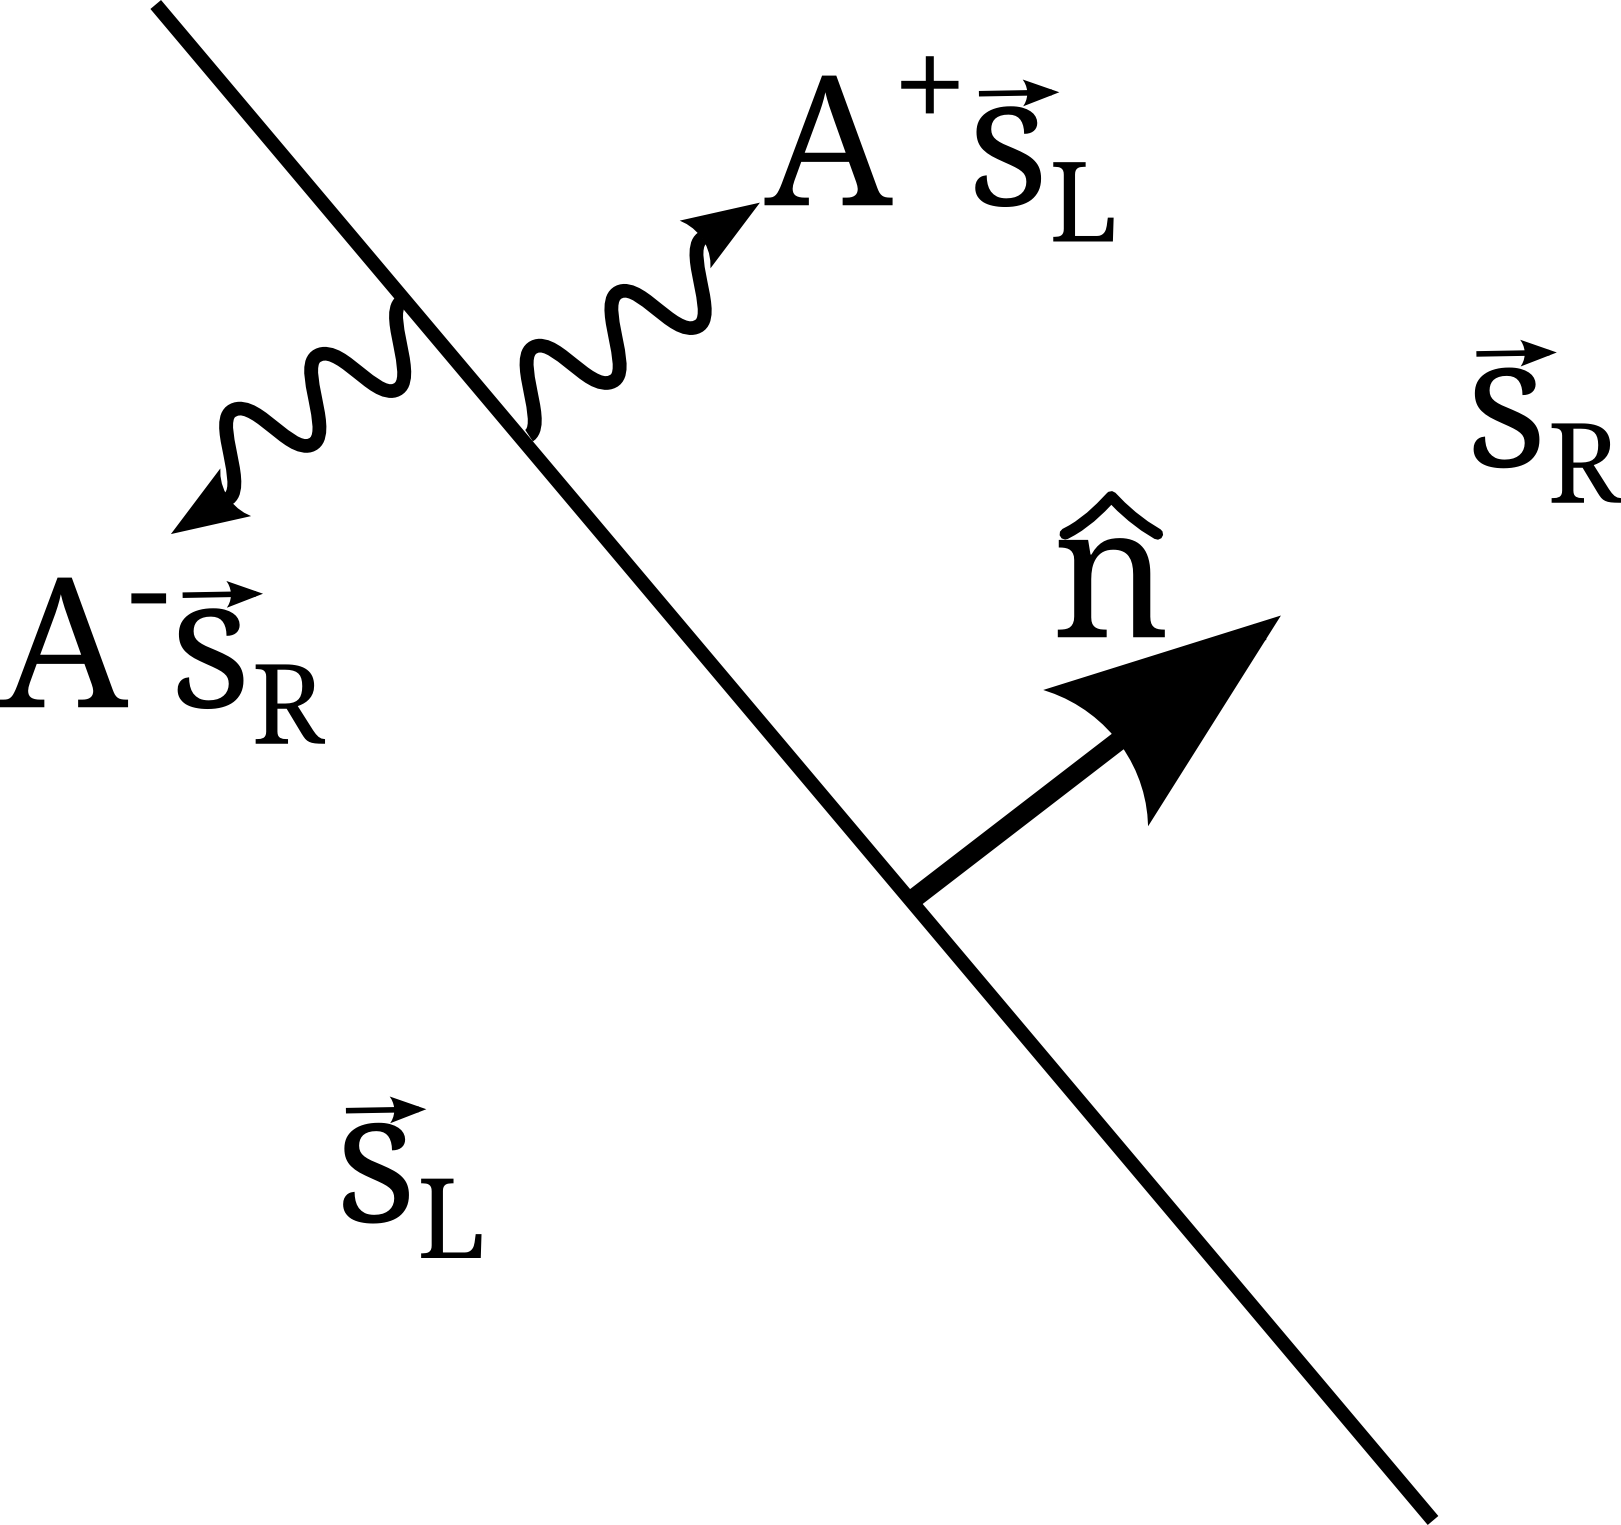
\includegraphics[width=0.4\textwidth]{figures/normalflux.png}
\caption{ A depiction of the setup for computing the flux across an edge. The flux is split by upwinding the characteristic variables of the Jacobian matrix. }\label{fig:normalflux}
\end{center}
\end{figure}
Regardless of which system we are solving, the DG approximation requires that we compute an estimate of the flux across an element's edge given the solution on either side of the edge. In general, the solution is discontinuous across the edges. Let $\vec{s}_L$ and $\vec{s}_R$ denote the solution to the ``left'' and to the ``right'' of the edge as depicted in Fig. \ref{fig:normalflux}. The goal is to compute the flux across an edge given the left and right states. The conservation law, \eqref{eq:conservationlaw}can be written
\begin{equation}
\vec{s}_t + \frac{\partial f^n}{\partial \vec{s}}\frac{\partial \vec{s}}{\partial n} = 0,
\end{equation}
where, for the sake of exposition, the source term has been dropped. The flux in the edge-normal direction is $f^n = \vec{f} \cdot \hat{n}$ and the directional derivative of the solution is $\frac{\partial \vec{s}}{\partial n}$. For a short period of time, $\Delta t$,
\begin{equation}
\vec{s}_t + \frac{\partial f}{\partial \vec{s}}|_{t=t_0} \frac{\partial \vec{s}}{\partial n}  = \mathcal{O}(\Delta t). \label{eq:linearizedForm}
\end{equation}
In \eqref{eq:linearizedForm}, the \textit{Jacobian} of the flux, $\frac{\partial f^n}{\partial \vec{s}}$, is evaluated at the fixed time $t=t_0$. For hyperbolic problems, like the shallow water equations, the Jacobian has real eigenvalues and can be diagonalized. Let
\begin{equation}
\frac{\partial f}{\partial \vec{s}}|_{t=t_0} = \boldsymbol{P} \boldsymbol{D} \boldsymbol{P}^{-1},\label{eq:diagonalized}
\end{equation} 
define the diagonalization, where $\boldsymbol{P}$ is a matrix whose columns are the eigenvectors and $\boldsymbol{D}$ is a diagonal matrix whose diagonal elements are the corresponding eigenvalues of the Jacobian. Substituting \eqref{eq:diagonalized} into \eqref{eq:linearizedForm} and multiplying on the left by $\boldsymbol{P}^{-1}$ gives
\begin{equation}
\vec{w}_t + \boldsymbol{D} \boldsymbol{P}^{-1}\frac{\partial \vec{s}}{\partial n}  = \mathcal{O}(\Delta t), \label{eq:diagForm}
\end{equation}
where $\vec{w} = P^{-1}\vec{s}$ are the \textit{characteristic} variables. Equation \eqref{eq:diagForm} can be rewritten, approximately as
\begin{equation}
\vec{w}_t + \boldsymbol{D} \frac{\partial \vec{w}}{\partial n}  \approx \mathcal{O}(\Delta t). \label{eq:diagonalizedForm}
\end{equation}
where variations in the eigenvectors with $n$ have been ignored. Equation \eqref{eq:diagonalizedForm} has approximate solutions
\begin{equation}
w^i = w^i_0( n - \lambda_i (t-t_0)) \label{eq:characteristicSolution}
\end{equation}
where $w^i$ and $\lambda_i$ are the $i^{th}$ eigenvector and eigenvalue, $w^i_0$ is the characteristic variable at time $t=t_0$, and $n$ is the physical distance normal to the edge. To evaluate the flux at the edge, we need to know the solution at the edge ($n=0$). At time $t_0 + \Delta t$,
\begin{equation}
w^i(0, \Delta t) = w^i_0(-\lambda_i\Delta t)
\end{equation}  
so that if $\lambda_i > 0$, the solution depends on the state to the left of the edge, and if $\lambda_i < 0$, the solution depends on the initial state to the right of the edge. Because of this, we split the diagonalization into two components,
\begin{equation}
\frac{\partial f}{\partial \vec{s}}|_{t=t_0} = \boldsymbol{P} \boldsymbol{D}^{+} \boldsymbol{P}^{-1} + \boldsymbol{P} \boldsymbol{D}^{-} \boldsymbol{P}^{-1} = \boldsymbol{A}^{+} + \boldsymbol{A}^{-},\label{eq:diagonalized-split}
\end{equation}
where $\boldsymbol{D}^{+}$ is the diagonal matrix with only positive eigenvalues and $\boldsymbol{D}^{-}$ is the diagonal matrix with only negative eigenvalues. The compact notation $\boldsymbol{A}^{+}$ and $\boldsymbol{A}^{-}$ is used for the Jacobian matrix associated with the splitting of the positive and negative eigenvalues. 

Under similar assumptions used to obtain \eqref{eq:characteristicSolution}, the flux at the boundary can be approximated
\begin{equation}
\vec{f}^n \approx \vec{f}^{n,*} = A^{+}\vec{s}_L + A^{-}\vec{s}_R  \label{eq:fluxApprox}
\end{equation}
It can be shown that
\begin{subequations}
\begin{align}
A^{+} &= \frac{A+|A|}{2} \\
A^{-} &= \frac{A-|A|}{2}
\end{align}
\end{subequations}
so that \eqref{eq:fluxApprox} can be written
\begin{equation}
\vec{f}^{n,*} = \frac{1}{2}\left( \vec{f}^n(\vec{s}_L) + \vec{f}^n(\vec{s}_R) -|A|(\vec{s}_L - \vec{s}_R) \right)\label{eq:RiemannFlux}
\end{equation}
Equation \eqref{eq:RiemannFlux} is the approximate Riemann flux. The choice of approximation for $|A|$ yields different linear flux schemes. In the shallow water software, we use the Lax-Friedrich's flux where $|A|$ is approximated by the maximum eigenvalue using either the left or the right state,
\begin{equation}
|A| = max( \lambda_i(\vec{s}_L), \lambda_i(\vec{s}_R) ).
\end{equation}


\subsection{Comparison with other SEM-Shallow Water Models}
The discretization presented here distinguishes itself from previous shallow water models presented in the literature. The models of \citet{Iskandarani1995} (and Ma1993) make use of the Gauss-Lobatto quadrature points, which were shown in \citet{Kopriva2006} to not satisfy the discrete metric identities and lead to the introduction of spurious modes associated with isoparametric elements. Here, the more accurate Gauss quadrature is used. The increased accuracy and satisfication of the discrete metric identities increases the algorithm cost. Since the Gauss quadrature points do not include the element boundaries, an additional step ( with $\mathcal{O}(N^2)$ operations per element ) is needed to interpolate the solution to the element boundaries before computing Riemann fluxes. An adpative filtering procedure, similar to \citet{Flad2016} is used for maintaining stability when marginally resolved modes violate energy conservation. In this way, the filter lowers the accuracy of the method only in locations where the solution is marginally resolved; the gain in performing the filtering is that numerical stability is maintained. This filtering procedure is different than \citet{Taylor1997} where the filter is applied everywhere at each time step. In the conservative form of the shallow water equations, care was taken in the computation of the bathymetry gradient to guarantee that a motionless fluid remains motionless to machine precision.

\chapter{Getting Started With an Example}
The easiest way to get started with the SELF Shallow Water software is run a pre-configured example. Doing so will introduce you to compiling, running, run-time configuring, and viewing the output. Once you are comfortable with a workflow for the example and you are ready to set up the software for your particular experiment, it may be beneficial to browse through other pre-configured examples to find one that is closest to the setup you have in mind. From there, modifications to the code can be made. Details on some of the more important routines and those you are likely to modify are provided in Chapter \ref{chap:Mods}.

\section{Downloading}
The SELF is currently available on github. There are two ways to obtain the code. If you are interested in obtaining the most recent snapshot of the code, a tar file can be downloaded directly from the git website.  \href{https://github.com/schoonovernumerics/SELF}{Clicking here will bring you to the SELF.} Once you follow the link ( if the embedded link doesn't work, copy and paste
\begin{verbatim}
 https://github.com/schoonovernumerics/SELF 
\end{verbatim}
into your browser's url bar ) click on ``Download ZIP'', which is located towards the right side of the page. Unpack the tar file into your favorite directory. This will make a directory ``SELF'' in your favorite directory, underneath which all of the source code and examples included with the SELF. 

Alternatively, if you have git installed on your computer, you can clone the SELF repository by issuing the command
\begin{center}
\begin{verbatim}
git clone https://github.com/schoonovernumerics/SELF
\end{verbatim}
\end{center}
Again, this will make the directory ``SELF'' in the current directory where you issued the clone command. 

\section{Compile the example}
At this point, you should have downloaded the SELF. We will first navigate to the examples directory and find the example for the ``shelf-steepening'' demo. This example can be found under
\begin{center}
\begin{verbatim}
SELF/examples/shallowwater/shelfsteepening/
\end{verbatim}
\end{center}
Go ahead and change directories to this example.

As with all of the supplied examples, there are three subdirectories
\begin{center}
\begin{verbatim}
build/     localmods/    run/
\end{verbatim}
\end{center}
This subdirectory structure is used in order to keep your model output, source code modifications, and model build details separate. For now we won't worry about the \texttt{localmods/} subdirectory; this subdirectory will be discussed later in Chapter \ref{chap:Mods} where we will illustrate how to modify the source code if needed for your application.

Right now, the most important thing is to get you familiar with compiling and running the code. Change directories into the build subdirectory. Underneath the build directory, there is a makefile and a simple build script. For now, you don't need to worry about changing anything to either one of these files. In Sec. \ref{sec:config}, there are directions for changing your fortran compiler, compiler optimizations, warning flags, debugging flags, etc. To compile the code, simply type the command
\begin{verbatim}
./rebuild.sh
\end{verbatim}
and press enter. This will compile all of the necessary modules and  driver programs (all of the dependencies are expressed in the makefile) and will generate two executables, \texttt{initialize\_sw} and \texttt{integrate\_sw}. Additionally, the \texttt{rebuild} script cleans up the build directory by removing the \texttt{.o} and \texttt{.mod} files and moves the executable to the run directory. If you have problems running the build script, it may be that the permissions are not set appropriately. To set the proper permissions, do
\begin{verbatim}
chmod 755 rebuild.sh
\end{verbatim}
and then try to run the script again. If this still doesn't work, send me an e-mail, and, for now, issue the commands
\begin{verbatim}
make initialize_sw
make integrate_sw
make clean
mv initialize_sw integrate_sw ../run/
\end{verbatim}

\section{Running the Code and Viewing the Output}
Ok, so now you have successfully compiled the code. Change directories to the \texttt{run} directory. In the run directory, you will find the executables (\texttt{initialize\_sw} and \texttt{integrate\_sw}), a SpecMesh file (\texttt{box.mesh}), and a text file ( \texttt{shallowwater.params} ).

\subsection{Running the Code}
Both executables require that you have a namelist file in the directory named \texttt{shallowwater.params}. There should be one included already with your fresh download. This namelist file specifies parameters that are used for the explicit time stepping, spatial discretization, and plotting and sets physical parameters relevant to the shallow water model. If you like, feel free to take a look at the file to familiarize yourself with the parameters, but don't worry about setting anything; the provided parameters file yields a successful run for this example. In Sec. \ref{sec:config}, we will discuss each parameter.

The work-flow for conducting a simulation is divided into two steps. The first step is the initialization. In the initialization phase, the model grid, bathymetry, forcing terms, and initial conditions are specified. The details of how this is done can be seen in the program \texttt{shelfsteepening/localmods/ShallowWater\_InitialConditions.f90}. 

To run the initialization program, execute
\begin{verbatim}
./initialize_sw
\end{verbatim}
 Once it finishes running, there will be three files that are generated:
\begin{enumerate}
\item \texttt{mesh.tec} : A tecplot file that contains the computational mesh and metric terms that were used in the computation of the solution.
\item \texttt{ShallowWater.init.tec} : A tecplot file that contains the initial conditions that are set in \texttt{ShallowWater\_InitialConditions.f90}
\item \texttt{ShallowWater.0000000000.pickup} : A ``pickup'' file that contains the necessary data to initialize the forward integration of the model.
\end{enumerate}

The \texttt{.tec} files can be viewed in VisIt or your favorite visualization software that can read TecPlot files. For this example, the model has already been tested and the initial configuration has been deemed acceptable for the physical problem in quetion. At this point in the work-flow, though, is usually when you would take a look at the initial conditions, the model grid, and the metric terms and verify that the setup is acceptable. Once you are happy with the initial condition configuration, it is time to move on to the forward integration phase.

At this point, it is relevant to discuss three of the parameters in the \texttt{shallowwater.params} file.
\begin{enumerate}
\item \texttt{iterInit} : This is the initial iterate, specified as an integer. This integer corresponds to the iteration stamp of the pickup file that you intend to read in. The iteration stamp is an integer that is padded with enough zeros to yield 10 digits.
\item \texttt{nTimeSteps} : This is the number of time steps that the integration program will execute. At the end of execution, the integration program will create a pickup file with an iteration stamp corresponding to \texttt{iterInit}+\texttt{nTimeSteps}.
\item \texttt{dumpFreq} : This is the frequency at which tecplot files are written.
\end{enumerate} 
These parameters, if you have not modified them, are set as
\begin{verbatim}
iterInit = 0,
nTimeSteps = 5000,
dumpFreq = 1000,
\end{verbatim}
so that the integration will begin with the pickup file generated from the initialization program, 5000 time steps will be executed, and a tecplot file will be generated every 1000 time steps. To run the integration program, do
\begin{verbatim}
./integrate_sw
\end{verbatim}
Once the program completes, you will see six new tecplot files and a new pickup file (\texttt{ShallowWater.0000005000.pickup}). The new pickup file can be used as a new initial condition if you wish to continue integrating past 5000 time steps, by setting 
\begin{verbatim}
iterInit = 5000,
\end{verbatim}

At this point, you have successfully compiled and completed the initialization and forward integration steps in the work-flow. This is a good time to discuss visualization before we discuss making modifications to the run-time parameters in \texttt{shallowwater.params}.

\subsection{Viewing the output in VisIt}
Now that the code has finished running and you have some output, you can view the tecplot and curve files in your favorite visualization software. Here, we will describe how to view the output using \href{https://wci.llnl.gov/simulation/computer-codes/visit/}{VisIt}.


\section{Configuration}\label{sec:config}


\chapter{Making modifications}\label{chap:Mods}


%\chapter{Testing the Linear Form}
%The linear shallow water equations without planetary rotation support gravity waves. Constant planetary rotation can lead to inertia-gravity waves. Near a no-normal flow boundary, Kelvin waves can arise that travel at the gravity wave speed and have an ``offshore'' decay scale equivalent to the \textit{deformation radius}. By introducing variable bathymetry with planetary rotation, topographic waves can arise that propagate due to the conservation of potential vorticity. A similar wave, known as a Rossby wave, can propagate due to variation of the coriolis parameter. In the following sections, the behavior of each of these waves is detailed and numerical solutions are presented in the form of refinement studies. It will be shown that the NDGSEM solution converges spectrally under p-refinement, consistent with the error analysis theory for a spectral method. Additionally, it will be shown that the NDGSEM produces the appropriate wave speeds and with minimal dissipation.


%\section{Gravity Waves}
%\subsection{Plane Wave Propagation}
%\subsection{Double Slit Experiment}

%\section{Geostrophic Adjustment}

%\section{Kelvin Wave Propagation}

%\section{Rossby Wave Propagation}

%\chapter{Testing the Nonlinear Conservative Form}

%\chapter{Testing the Nonlinear Skew-Symmetric Form}


\clearpage

\appendix

%\chapter{Spectral Element Primer}

%\section{Vector Spaces}


%\section{Spectral Approximations and Error Analysis}

%\chapter{Differential Geometry}\label{chap:GeometryTheory}

\pagebreak

\bibliography{hpe-refs}
\bibliographystyle{plainnat}
\end{document}